\chapter{Desarrollo}

El cuerpo principal de la memoria describe el trabajo realizado.
En este ejemplo, demostramos algunas construcciones típicas: una
cita bibliográfica~\parencite{knuth1986} y referencias cruzadas a
la sección~\ref{sec:arquitectura}. La cita anterior es parentética
(autor y año dentro del paréntesis); cuando el autor ya forma parte
de la frase conviene usar \verb|\textcite|, que sólo encierra el
año: \textcite{tolkien1954lord} cuenta cómo Bilbo decía a menudo
que solo había un camino y que era como un río caudaloso; nacía
en el umbral de todas las puertas, y todos los senderos eran ríos
tributarios. ``Es muy peligroso, Frodo, cruzar la puerta'', solía
decirme. ``Vas hacia el Camino, y si no cuidas tus pasos no sabes
hacia donde te arrastrarán''.

Las imágenes se guardan en la carpeta \texttt{img/} y se incluyen con
\verb|\includegraphics| dentro de un entorno \texttt{figure}, que les
añade un pie y una etiqueta para poder referenciarlas, como en la
figura~\ref{fig:bolson-cerrado}. Conviene dar el ancho en relación con
\verb|\textwidth| y se puede omitir la extensión del archivo. Si la
imagen no es propia, el pie debe indicar su autoría y procedencia.

\begin{figure}
  \centering
  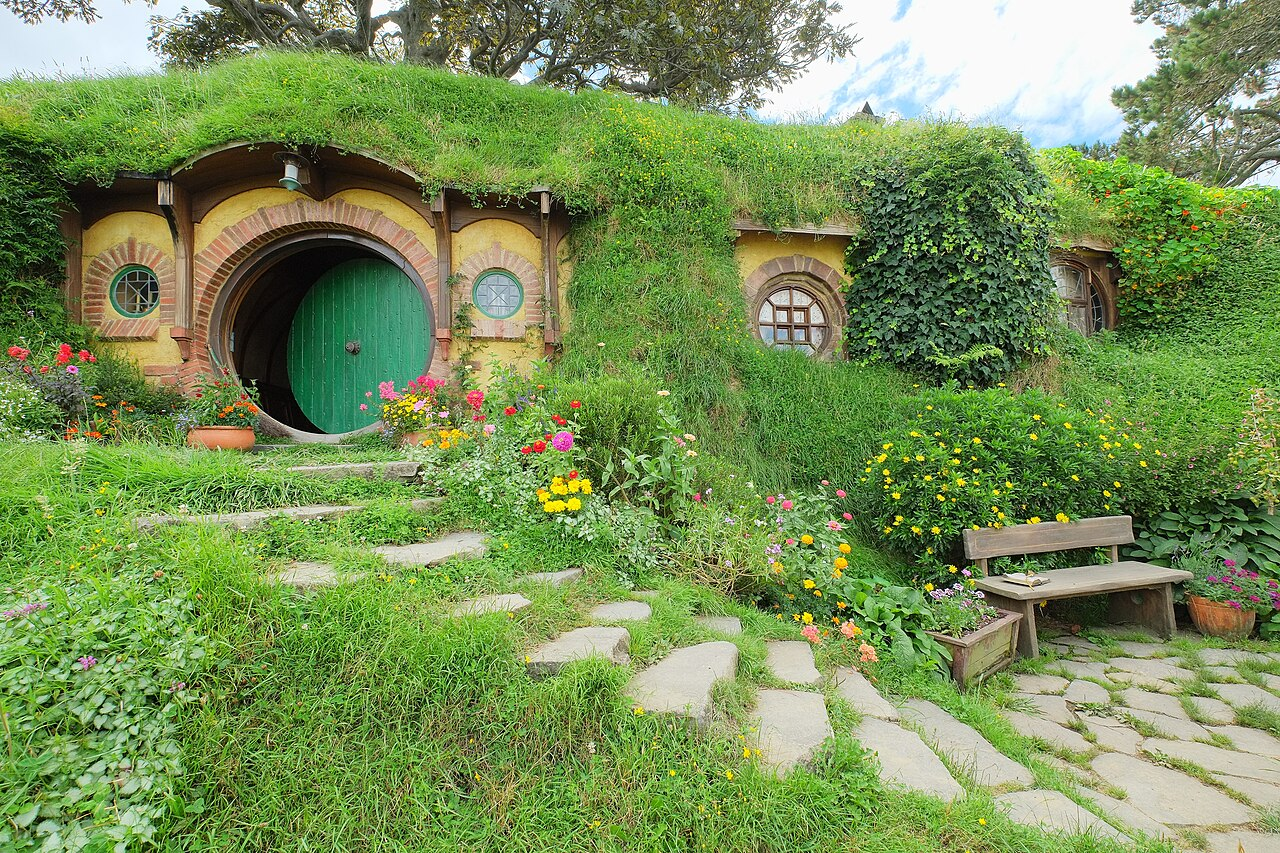
\includegraphics[width=0.8\textwidth]{img/bolson_cerrado}
  % El argumento opcional es la versión corta para el índice de figuras.
  \caption[Bolsón Cerrado]{Bolsón Cerrado, residencia de los Bolsón, en
    el decorado de Hobbiton (Matamata, Nueva Zelanda). Fotografía de
    Pseudopanax (2018), en dominio público. Fuente: Wikimedia Commons,
    \url{https://commons.wikimedia.org/wiki/File:Baggins_residence_'Bag_End'.jpg}.}
  \label{fig:bolson-cerrado}
\end{figure}

\section{Arquitectura}
\label{sec:arquitectura}

La arquitectura del sistema sigue el patrón de separación entre
normativa y estilo. La clase \texttt{fdi-simplex} implementa los
requisitos obligatorios de la normativa UCM-FDI; el aspecto
visual concreto queda delegado a la opción \texttt{estilo}, como
resume la tabla~\ref{tab:estilos}. Las tablas se componen con el entorno
\texttt{tabular} dentro de un \texttt{table} que, igual que
\texttt{figure}, es un flotante: \LaTeX{} decide dónde colocarlo, y
no siempre queda junto al texto que lo menciona.

\begin{table}
  \centering
  \begin{tabular}{|l|l|}
    \hline
    \textbf{Estilo} & \textbf{Descripción} \\
    \hline
    \texttt{digital} & Lora, enlaces en color, pensado para leer en pantalla \\
    \hline
    \texttt{clasico} & Reminiscente de TeXiS, a dos caras \\
    \hline
    \texttt{minimo} & Casi sin personalizar, para partir de él \\
    \hline
  \end{tabular}
  \caption{Estilos disponibles en la clase.}
  \label{tab:estilos}
\end{table}

\section{Implementación}

La implementación se basa en la clase KOMA-Script
\texttt{scrbook} \autocite{kohm2004koma}, con soporte nativo para UTF-8 mediante
LuaLaTeX.
